\chapter{ROS and Tensorflow}

	\section{Overview of ROS}
	\label{sec:Overview of ROS}
		ROS (\emph{Robot Operating System})~\cite{ros} is a BSD-licensed system for controlling robotic components from a PC. A ROS system is comprised of a number of independent nodes, each of which communicates with the other nodes using a publish/subscribe messaging model. For example, a particular sensor’s driver might be implemented as a node, which publishes sensor data in a stream of messages. These messages could be consumed by any number of other nodes, including filters, loggers, and also higher-level systems such as guidance, pathfinding, etc.
		
		\textbf{Why ROS?}
		
		Nodes in ROS do not have to be on the same system (multiple computers) or even of the same architecture. We can have a Arduino publishing messages, a laptop subscribing to them, and an Android phone driving motors. This makes ROS really flexible and adaptable to the needs of the user. ROS is also open source, maintained by many people. This is of prime importance in this thesis work.
		
		Let’s say we have a camera on our Robot. We want to be able to see the images from the camera, on another laptop. The Camera Node takes care of communication with the camera, Image Processing Node on the robot processes image data, and a Image Display Node displays images on a screen. To start with, all Nodes have registered with the Master. The Master is like a lookup table where all the nodes go to find where exactly to send messages.
		
		\begin{figure}[htbp]
			\centering
			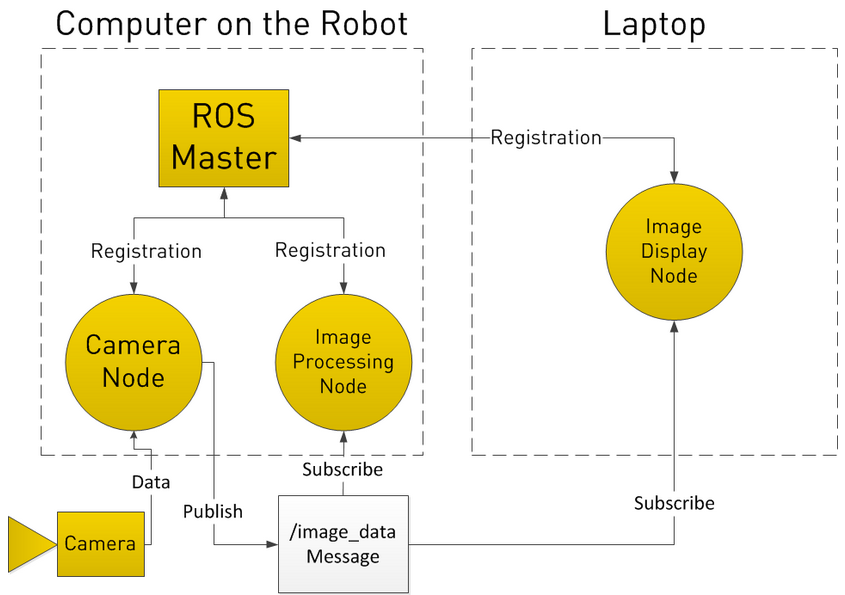
\includegraphics[width=12cm]{ROS_working.png}
			\caption{ROS working\label{ROS working}}
		\end{figure}
		
		In registering with the ROS Master, the Camera Node states that it will Publish a Topic called \emph{/image-data} (for example). Both of the other Nodes register that they are Subscribed to the Topic \emph{/image-data}.
		
		Thus, once the Camera Node receives some data from the Camera, it sends the \emph{/image-data} message directly to the other two nodes, on different computer or to the onboard computer.(Through TCP/IP usually)
	
	
	\section{Basics of Tensorflow}
	\label{sec:Basics of Tensorflow}
		TensorFlow is a framework created by Google for creating Deep Learning models~\cite{abadi2016tensorflow}. Deep Learning is a category of machine learning models that use multi-layer neural networks. The idea of deep learning has been around since 1943 when neurophysiologist Warren McCulloch and mathematician Walter Pitts wrote a paper on how neurons might work and they modeled a simple neural network using electrical circuits.
		
		\newpage
		\noindent\textbf{Basic Computational Graph}

		\noindent Everything in TensorFlow is based on creating a computational graph. Here we have a computational graph as a network of nodes, with each node known as an operation, running some function that can be as simple as addition or subtraction to as complex as some multi variate equation.
		
		In a TensorFlow graph, each node has zero or more inputs and zero or more outputs, and represents the instantiation of an operation. Values that flow along normal edges in the graph (from outputs to inputs) are tensors,
		arbitrary dimensionality arrays where the underlying element type is specified or inferred at graph-construction time. Special  edges,  called
		control  dependencies, can also exist in the graph:  no data flows along such edges, but they indicate that the source node for the control dependence  must  finish  executing  before  the  destination node for the control dependence starts executing.
		
		\begin{figure}[htbp]
			\centering
			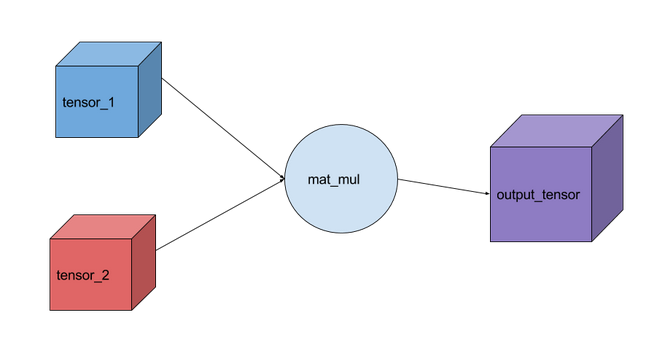
\includegraphics[width=12cm]{computation.png}
			\caption{Our computation graph\label{Our computation graph}}
		\end{figure}
		
		An Operation also referred to as op can return zero or more tensors which can be used later on in the graph.Each operation can be handed a constant, array, matrix or n-dimensional matrix. Another word for an n-dimensional matrix is a tensor, a 2-dimensional tensor is equivalent to a m x m matrix.
		
		Clients programs interact with the TensorFlow system by creating a
		Session. To create a computation graph, the Session interface supports an
		Extend method to augment the current graph managed by the session with additional nodes and edges (the initial graph when a session is created is empty).
		
		\noindent\textbf{Implementation}
		
		\noindent The  main  components  in  a  TensorFlow  system  are  the client, which uses the Session interface to communicate with the master, and one or more
		worker processes, with each worker process responsible for arbitrating access to one or more computational devices(such as CPU cores or GPU cards) and for executing graph nodes on those devices  as  instructed  by  the  master. We  have  both local and distributed implementations of the TensorFlow interface. The  local  implementation  is  used  when  the
		client, the master, and the worker all run on a single machine in the context of a single operating system process (possibly with multiple devices, if for example, the machine  has  many  GPU  cards  installed).   The  distributed implementation shares most of the code with the local
		implementation,  but  extends  it  with  support  for  an  environment where the client, the master, and the workers can all be in different processes on different machines.
		
%		\begin{figure}[htbp]
%			\centering
%			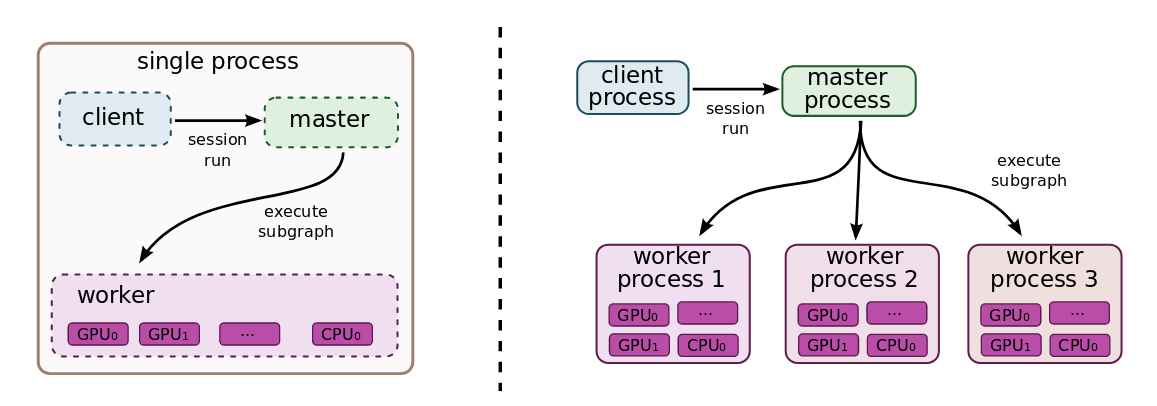
\includegraphics[width=16cm]{tensorimg.png}
%			\caption{Single machine and distributed system structure\label{Single machine and distributed system structure}}
%		\end{figure}
	
	
	
	
	
	
	
	